\section{An Infrastructure for Non-functional Testing Using Docker Containers}

To allow code generator testing, we need to deploy the test harness, \ie the produced binaries, on an elastic infrastructure that provides preconfigured virtual server images, storage, and resources that may be provisioned by testers. 
Monitoring information should also be provided to inform about resource utilization required/needed and to automate the resource management of deployed components. 
For this purpose, we propose a testing infrastructure based on System Container techniques such as Docker\footnote{\url{https://www.docker.com}} environment. 

Docker will automate the deployment of applications inside software containers. It will simplify the creation of highly distributed systems by allowing multiple applications to run autonomously on a server (basically a cloud server). 
Docker provides a platform as a service (PaaS) style of deployment for software programs. 
Consequently, we rely on this technology and benefit from all its advantages to:
\begin{enumerate}
	\item Deploy generated code within Docker containers
	\item Automate optimization sequences generation
	\item Monitor service containers
	\item Gather performance metrics (CPU, Memory, I/O, etc.)
\end{enumerate}

We integrate a collection of Docker components to define the adequate infrastructure for testing and monitoring of code generators. 
In the following sections, we describe the deployment and testing architecture of generated code within Docker.

\subsection{System Container as Deployment Environment}

Before starting to monitor and test applications, we have to deploy generated code on different components to ease containers provisioning and profiling.
We aim to use Docker Linux containers to monitor the execution of produced binaries by GCC compilers in term of resource usage. 
Docker is an open source engine that automates the deployment of any application as a lightweight, portable, and self-sufficient container that runs virtually on a host machine. 
To achieve that, Docker uses the Linux container technology. The main advantages that Docker offers compared to using a full stack virtualization solution is less performance overhead and resource isolation. 

Using Docker, we can define preconfigured applications and servers to host. We can also define the way the service should be deployed in the host machine. 
As properties, we can define the OS where the service has to run, dependencies, etc. Once Docker images are defined, we can instantiate different containers.
A simple way to define Docker images is to use Dockerfiles. Docker can build images automatically by reading the instructions from a Dockerfile. 
Therefore, for our experiments we describe a Dockerfile that defines the target compiler to test, as well the container OS. The same Docker image will be used then, to execute different instances of generated code. Basically, each container deploys an optimized version of the input source code program.

Docker uses as well Linux control groups (cgroups) to group processes running in the container. This allows us to manage the resources of a group of processes, which is very valuable. 
This approach increases the flexibility when we want to manage resources, since we can manage every group individually. 

Therefore, to run our experiments, each optimized program is executed individually inside an isolated Linux container. By doing so, we ensure that each executed program runs in isolation without being affected by the host machine or any other processes. Moreover, since a container is cheap to create, we are able to create too many containers as long as we have new programs to execute.

Since each program execution requires a new container to be created, it is crucial to remove and kill containers that have finished their job to eliminate the load on the system. In fact, containers/programs are running sequentially without defining any constraints on resource utilization for each container. So once execution is done, resources reserved for the container are automatically released to enable spawning next containers. Therefore, the host machine will not suffer too much from the performance trade-offs.

\subsection{Runtime Testing Components}
In order to test our running applications within Docker containers, we aim to use a set of Docker components to ease the extraction of non-functional properties.
\subsubsection{Monitoring Component}
This container will provide us an understanding of the resource usage and performance characteristics of our running containers. Generally, Docker containers rely on cgroups file systems to expose a lot of metrics about accumulated CPU cycles, memory, block I/O usage, etc. Therefore, our monitoring component automates the extraction of runtime performance metrics using cgroups. For example, we access to live resource consumption of each container available at the cgroup file system via stats found in $/sys/fs/cgroup/cpu/docker/(longid)/$ (for CPU consumption) and $/sys/fs/cgroup/memory/docker/(longid)/$ (for stats related to memory consumption). This component will automate the process of service discovery and metrics aggregation so that, instead of gathering manually metrics located in cgroups file systems, it will extract automatically runtime resource usage statistics relative to running components. We note that resource usage information is collected in raw data. This process may induce a little overhead, because it does very fine-grained accounting of resource usage on running container. Fortunately, this may not affect the gathered performance values since we run only one generated program by GCC within each container.

To ease the monitoring process, we use google containers called cAdvisor as Container Advisor\footnote{https://github.com/google/cadvisor}. It is a tool developed by Google to monitor their infrastructure. 
cAdvisor Docker image does not need any configuration on the host machine. We have just to run it on our Docker host. It will then have access to the resource usage and performance characteristics of all running containers. This image uses the cgroups mechanism described above to collect, aggregate, process, and export ephemeral real-time information about running containers. Then, it reports all statistics via web UI ($http://localhost:8080$) to view live resource consumption of each container. cAdvisor has been widely in different projects such as Heapster\footnote{https://github.com/kubernetes/heapster} and Google Cloud Platform\footnote{https://cloud.google.com/}.

However, cAdvisor monitors and aggregates live data over only 60 seconds interval. Therefore, we would like to record all data over time since container's creation. This is useful to run queries and define non-functional metrics from historical data. Thereby, To make gathered data truly valuable for resources usage monitoring, it becomes necessary to log it in a database at runtime. Thus, we link our monitoring component to a back-end database for better understanding of non-functional properties. 
\subsubsection{Back-end Database Component}
This component represents a times-series database back-end. It is plugged with the previously described monitoring component to save the non-functional data for long-term retention, analytics and visualization. Hence, we define its corresponding ip port into the monitoring component so that, container statistics are sent over TCP port (e.g, 8083) exposed by the database component.

During the execution of generated code, resource usage stats will be continuously sent into this component. When a container is killed, all statistics will be deleted afterward. We choose a time series database because we are collecting time series data that corresponds to the resource utilization profile of generated code execution.

We use InfluxDB\footnote{https://github.com/influxdata/influxdb}, an open source distributed time series database as a back-end to record data. InfluxDB allows the user to execute SQL-like queries on the database. For example the following query reports the average memory usage of container $"generated\_code\_v1"$ for each 2s since container has started:

\begin{lstlisting}[
language=SQL,
showspaces=false,
basicstyle=\ttfamily,
numberstyle=\tiny,
commentstyle=\color{gray},
linewidth=\columnwidth
]
select mean(memory_usage) from stats where 
container_name='generated_code_v1' group by 
time(2s)
\end{lstlisting}
To give an idea about data stored in InfluxDB. The following table describes the different stored metrics:
 \begin{table}[h]
 	\begin{center}
 		\begin{tabular}{|p{1cm}|p{6.9cm}|}
 			\hline
 			 Name & Name of the container \\
 			\hline
 			 Ts & Starting time of the container in epoch time \\
 			\hline
 			 Network &  Stats for network bytes and packets in an out of the container \\
 			\hline
 			 Disk IO &  Disk I/O stats \\
 			\hline
 			 Memory &  Memory usage \\
 			
 			\hline
 		   	CPU &  Cumulative CPU usage \\
 			\hline
 			
 		\end{tabular}
 		
 	\end{center}
 	\caption {Resource usage metrics recorded in InfluxDB}
 	%\vspace*{-0.9cm}
 \end{table}

For instance, we set the back-end container of our component-based infrastructure. It would be nice to pull all pieces together to view resource consumption graphs within a complete dashboard. It is relevant to show performance profiles of memory and CPU consumption for example of our running applications overtime. To do that, we present a front-end visualization component for performance profiling. 
\begin{figure*}[h]
	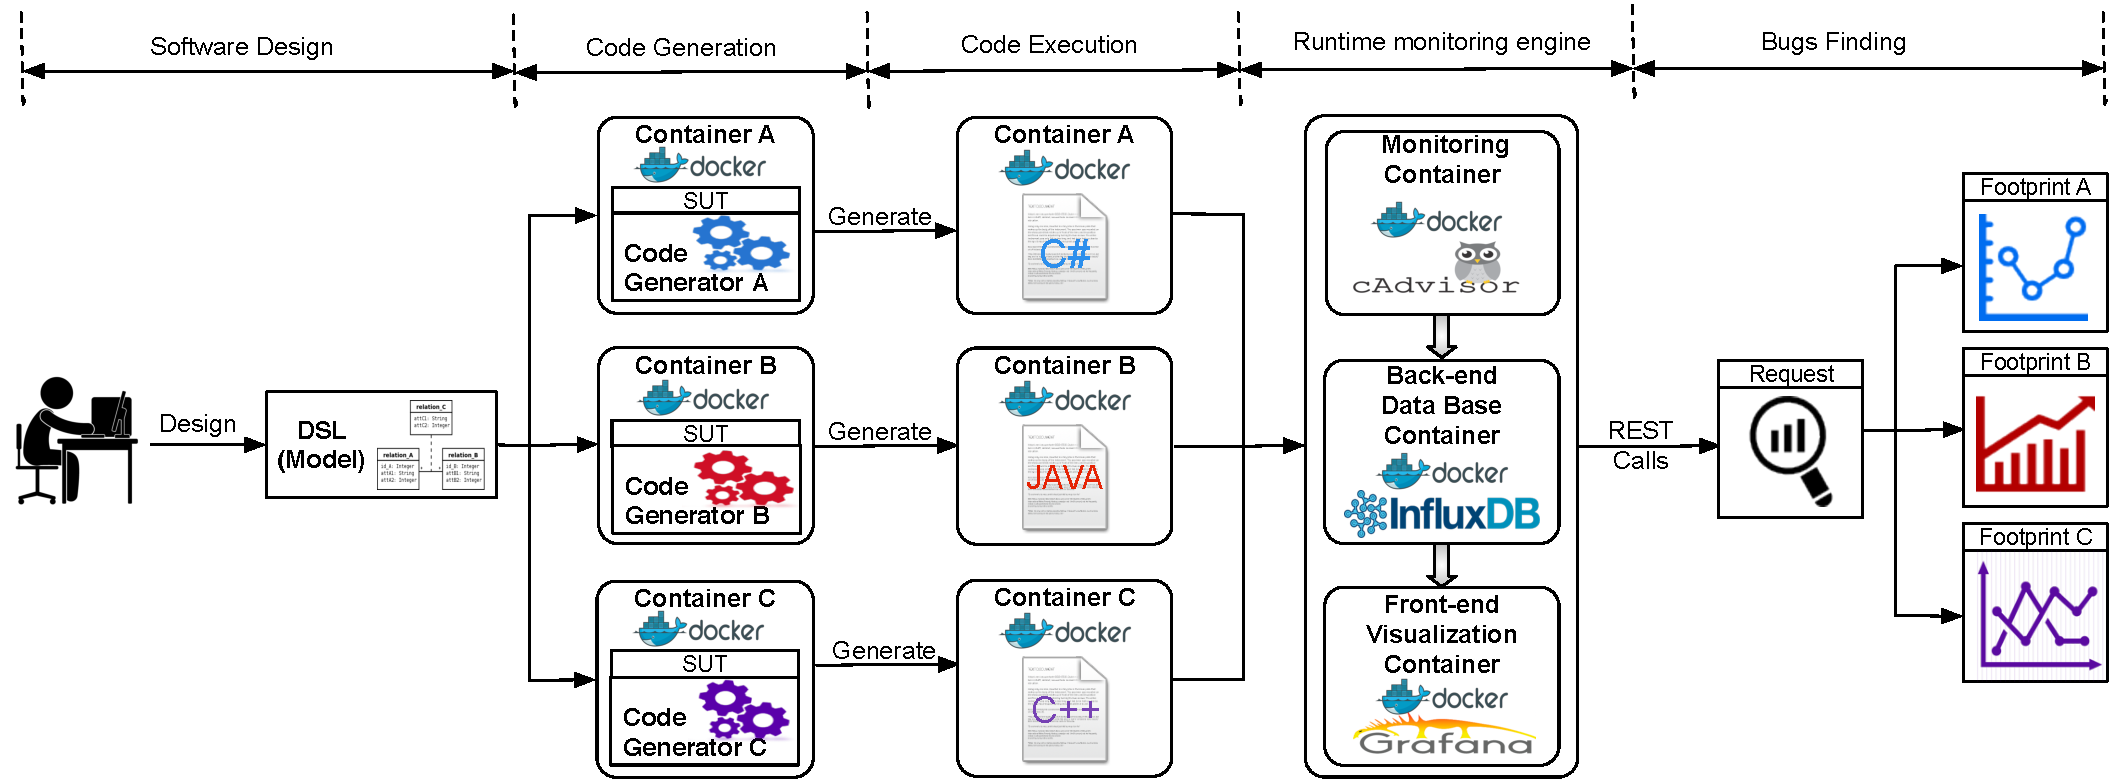
\includegraphics[width=1\linewidth]{Ressources/background2.pdf}
	\caption{An overall overview of the different processes involved to ensure the code generation and non-functional testing of produced code from design time to runtime.}
	%		\label{AAA}
\end{figure*}
\subsubsection{Front-end Visualization Component}
Once we gather and store resource usage data, the next step is visualizing them. That is the role of the visualization component. It will be the endpoint component that we use to visualize the recorded data. Therefore, we provide a dashboard to run queries and view different profiles of resource consumption of running components through web UI. Thereby, we can compare visually the profiles of resource consumption among containers. Moreover, we use this component to export the data currently being viewed into static CSV document. Thereby, we can perform statistical analysis on this data to detect inconsistencies or performance anomalies. An overview of the monitoring dashboard is shown in Figure 3.

To do so, we choose Grafana\footnote{https://github.com/grafana/grafana}, one of the best time-series metric visualization tools available for Docker. It is considered as a web application running within a container. We run Grafana within a container and we link it to InfluxDB by setting up the data source port 8086 so that it can easily request data from the database. 
We recall that InfluxDB also provides a web UI to query the database and show graphs. But, Grafana will let us to display live results over time in much pretty looking graphs. Same as InfluxDB, we use SQL queries to extract non-functional metrics from the database for visualization.

\subsection{Wrapping Everything Together: Architecture Overview}
To summarize, we present, as shown in Figure 1, an overall overview of the different components involved in our Docker monitoring infrastructure.




Our testing infrastructure will run different jobs within Docker containers. First, we generate and run different versions of code using our target compiler. To do so, we run multiple instances of our preconfigured Docker image that corresponds to specific code generator (e.g, GCC compiler). Each container will execute a specific job. For our case, a job represents a program compiled with new optimization sequence generated by NS. In the meanwhile, we start our runtime testing components (e.g., cAdvisor, InfluxDB and Grafana). The monitoring component collects usage statistics of all running containers and save them at runtime in the time series database component. The visualization component comes later to allow end users to define performance metrics and draw up charts.
